\setcounter{chapter}{10}
\chapter{Parametric Equations and Polar Coordinates}

\section{Curves Defined by Parametric Equations}

$x$ and $y$ are given as functions of a third variable $t$,
a \textbf{parameter}, by the equations

$$ x = f(t) \qquad y = g(t) $$

Each value of $t$ determines a point ($x$, $y$).
As $t$ varies, the point ($x$, $y$) = ($f(t)$, $g(t)$)
varies and traces out a curve $C$, a \textbf{parametric curve}.

\subsection*{Example}

Sketch the curve defined by
$$ x = t^2-2t \qquad y = t+1 $$

\subsection*{Solution}
Use values for $t$ and plug those into $x(t)$ and $y(t)$ to get points ($x$, $y$)

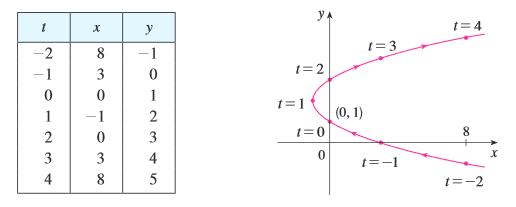
\includegraphics{example11-1-1}

\section{Calculus with Parametric Curves}

\subsection*{Tangents}
$f$ and $g$ are differentiable functions and we want to find the
tangent line at a point ($f(t)$, $g(t)$). The Chain Rule gives

$$ \frac{dy}{dt} = \frac{dy}{dx} \cdot \frac{dx}{dt} $$

$$ \frac{dy}{dx} = \frac{\frac{dy}{dt}}{\frac{dx}{dt}} \qquad if \: \frac{dx}{dt} \neq 0$$

$d^2y/dx^2$ can be found by replacing $y$ with $dy/dx$ in the equation above

$$ \frac{d^2y}{dx^2} = \frac{d}{dx}\left(\frac{dy}{dx}\right) = \frac{\frac{d}{dt}(\frac{dy}{dx})}{\frac{dx}{dt}} $$

\subsection*{Example}
Find the tangent to the cycloid $x=r(\theta - sin\: \theta)$, $y=r(1-cos\: \theta)$
at the point where $\theta=\pi/3$.

\subsection*{Solution}
The slope of the tangent is
$$\frac{dy}{dx}=\frac{dy/d\theta}{dx/d\theta}=\frac{r\: sin\: \theta}{r(1-cos\: \theta)}
    =\frac{sin\: \theta}{1-cos\: \theta}$$
When $\theta=\pi /3$, we have
$$x=r\left(\frac{\pi}{3}-sin\frac{\pi}{3}\right)=r\left(\frac{\pi}{3}-\frac{\sqrt{3}}{2}\right)
    \qquad y=r\left(1-cos\frac{\pi}{3}\right)=\frac{r}{2}$$
and
$$\frac{dy}{dx}=\frac{sin(\pi/3)}{1-cos(\pi/3)}=\sqrt{3}$$
Therefore the slope of the tangent is $\sqrt{3}$ and its equation is
$$y-\frac{r}{2}=\sqrt{3}\left(x-\frac{r\pi}{3}+\frac{r\sqrt{3}}{2}\right)$$

\subsection*{Areas}
Area under a curve $y = F(x)$ form $a$ to $b$ is $A = \int_a^b F(x) dx$.
If the curve is traced out with the parametric equations $f(t)$ and $g(t)$,
we can calculate the area by using the Substitution Rule for Definite Integrals:

$$A=\int_a^b ydx = \int_\alpha^\beta g(t)f'(t)dt$$

\subsection*{Example}
Find the area under one arch of the cycloid
$$x=r(\theta-sin\: \theta) \qquad y=r(1-cos\: \theta)$$

\subsection*{Solution}
One arch of the cycloid is given by $0\leq \theta \leq 2\pi$. Using the substitution
rule with $y=r(1-cos\: \theta)$ and $dx=r(1-cos\: \theta)d\theta$, we have
$$A=\int_0^{2\pi r}y\: dx=\int_0^{2\pi r}r(1-cos\: \theta)r(1-cos\: \theta)d\theta$$
$$=r^2(\frac{3}{2}\cdot 2\pi)=3\pi r^2$$

\subsection*{Arc Length}
To find the length $L$ of a curve $C$ in the from $y=F(x)$
$$ L = \int_a^b \sqrt{1+(\frac{dy}{dx})^2} dx $$

Suppose C can also be described with parametric equations, we obtain
$$ L = \int_a^b \sqrt{1+\left(\frac{dy}{dx}\right)^2} dx = \int_\alpha^\beta \sqrt{1+(\frac{dy/dt}{dx/dt})^2}\frac{dx}{dt}dt $$

\subsection*{Theorem}
If a curve C is described by the parametric equations $x=f(t)$, $y=g(t)$,
$\alpha \leq t \leq \beta$, where $f'$ and $g'$ are continuous on [$\alpha$,$\beta$]
and $C$ is traversed exactly once as $t$ increases from $\alpha$ to $\beta$, then
the length of $C$ is
$$ L = \int_a^b \sqrt{\left(\frac{dx}{dt}\right)^2+\left(\frac{dy}{dt}\right)^2} dt $$

\subsection*{Example}
Find the length of one arch of the cycloid $x=r(\theta-sin\theta)$, $y=r(1-cos\:\theta)$

\subsection*{Solution}
Since
$$\frac{dx}{d\theta}=r(1-cos\:\theta) \qquad \frac{dy}{d\theta}=rsin\:\theta$$
we have
$$L=\int_0^{2\pi}\sqrt{\left(\frac{dx}{d\theta}\right)^2+\left(\frac{dy}{d\theta}\right)^2}d\theta$$
$$=\int_0^{2\pi}\sqrt{r^2(1-cos\:\theta)^2+r^2sin^2\theta}d\theta$$
$$=r\int_0^{2\pi}\sqrt{2(1-cos\:\theta)}d\theta$$
$$=2r[2+2]=8r$$

\subsection*{Surface Area}
Suppose a curve $C$ is rotated about the $x$-axis. If $C$ si traversed exactly
once as $t$ increases from $\alpha$ to $\beta$, then the area of the surface is given by
$$ S = \int_\alpha^\beta 2 \pi y \sqrt{\left(\frac{dx}{dt}\right)^2+\left(\frac{dy}{dt}\right)^2} dt $$

The general symbolic formulas $S=\int 2 \pi y ds$ and $S = \int 2 \pi x ds$
are still valid, but for parametric curves we use
$$ ds = \sqrt{\left(\frac{dx}{dt}\right)^2+\left(\frac{dy}{dt}\right)^2} dt $$

\subsection*{Example}
Show that the surface area of a sphere of radius $r$ is $4\pi r^2$.

\subsection*{Solution}
The sphere is obtained by rotating the semicircle
$$x=rcos\:t \qquad y=rsin\:t \qquad 0\leq t\leq \pi$$
about the $x$-axis. Then, we get
$$S=\int_0^\pi 2\pi r\: sin\:t\sqrt{(-rsin\:t)^2+(rcos\:t)^2}dt$$
$$=2\pi r^2\int_0^\pi sin\:t\:dt = 2\pi r^2(-cos\:t)]_0^\pi = 4\pi r^2$$

\section{Polar Coordinates}
The Polar Coordinate System starts witha point in the plan called the \textbf{pole}
and is labeled $O$. Then we draw a ray starting at $O$ called the \textbf{polar axis}.
This corresponds to the positive $x$-axis in Cartesian coordinates. \par

$r$ is the ditsance from $O$ to $P$ and $\theta$ is the angle between the polar axis
and the line $OP$. The \textbf{polar coordinates} of $P$ are in the form ($r$, $\theta$), \par

If a point $P$ has Cartesian coordinates ($x$, $y$) and polar coordinates ($r$, $\theta$)
$$ cos \: \theta = \frac{x}{r} \qquad y = r sin \: \theta $$

and so
$$ x=r cos \: \theta \qquad y = r sin \: \theta$$

To find $r$ and $\theta$ when $x$ and $y$ are known, we use
$$ r^2 = x^2 + y^2 \qquad tan \: \theta = \frac{y}{x} $$

\subsection*{Example}
What curve is represented by the polar equation $r$=2?

\subsection*{Solution}
The equation $r$ = $a$ represents a circle with center $O$ and radius $|a|$.
The polar equation represents a circle about the origin with a radius of 2.

\subsection*{Example}
What curve is represented by the polar equation $\theta$=1?

\subsection*{Solution}
This curve consists of all points ($r$, $\theta$) such that $\theta$ is 1 radian.
It is a straight line that passes through $O$ and makes an angle of 1 radian with
the polar axis.

\subsection*{Tangents to Polar Curves}
To find a tangent line to a polar curve $r$ = $f(\theta)$, we write its parametric equations as
$$ x=r cos \: \theta=f(\theta)\:cos \: \theta \qquad y = r sin \: \theta = f(\theta)\:sin \: \theta$$

Then, using the method of finding slopes of parametric curves and the Product Rule, we have
$$ \frac{dy}{dx}=\frac{\frac{dy}{d\theta}}{\frac{dx}{d\theta}}=\frac{\frac{dr}{d\theta}sin\:
        \theta+r\:cos\:\theta}{\frac{dr}{d\theta}cos\:\theta-r\:sin\:\theta} $$

\section{Areas and Lengths in Polar Coordinates}

Using the formula for the area of a sector of a circle
$$ A=\frac{1}{2}r^2\theta $$

the formula for the area $A$ of the polar region $R$ is
$$ A=\int_a^b\frac{1}{2}[f(\theta)]^2 \: d\theta  = \int_a^b\frac{1}{2}r^2 \: d\theta$$

\subsection*{Arc Length}

To find the length of a polar curve $r$=$f(\theta)$, we write the parametric equations as
$$ x=r cos \: \theta=f(\theta)\:cos \: \theta \qquad y = r sin \: \theta = f(\theta)\:sin \: \theta$$

Using the Product Rule and differentiating with respect to $\theta$, we obtain
$$ \frac{dx}{d\theta}=\frac{dr}{d\theta}\:cos\:\theta-r\:sin\:\theta \qquad \frac{dy}{d\theta}=
    \frac{dr}{d\theta}\:sin\:\theta+r\:cos\:\theta $$

so, using $cos^2\theta + sin^2\theta = 1$, we have
$$ \left(\frac{dx}{d\theta}\right)^2 + \left(\frac{dy}{d\theta}\right)^2 = \frac{dr}{d\theta})^2 + r^2$$

Therefore the length of a curve is
$$ L=\int_a^b\sqrt{r^2+\left(\frac{dr}{d\theta}\right)^2}\:d\theta $$

\section{Conic Sections}

\subsection*{Parabolas}
An equation of the parabola with focus (0, $p$) and directrix $y=-p$ is
$$ x^2=4py $$

\subsection*{Ellipses}
The ellipse
$$ \frac{x^2}{a^2}+\frac{y^2}{b^2}=1 \qquad a \leq b > 0 $$
has focus ($\pm c$, 0), where $c^2=a^2-b^2$, and vertices ($\pm a$, 0) \\
The ellipse
$$ \frac{x^2}{b^2}+\frac{y^2}{a^2}=1 \qquad a \leq b > 0 $$
has focus (0, $\pm c$), where $c^2=a^2-b^2$, and vertices (0, $\pm a$)

\subsection*{Hyerpbolas}
The hyperbola
$$ \frac{x^2}{a^2}-\frac{y^2}{b^2}=1 $$
has foci($\pm c$, 0), where $c^2=a^2+b^2$, vertices ($\pm a$, 0), and
asymptomes $y=\pm(b/a)x$. \\
The hyperbola
$$ \frac{y^2}{a^2}-\frac{x^2}{b^2}=1 $$
has foci(0, $\pm c$), where $c^2=a^2+b^2$, vertices (0, $\pm a$), and
asymptomes $y=\pm(a/b)x$.

\section{Conic Sections in Polar Coordinates}

\subsection*{Theorem}
Let $P$ be a fixed point (the \textbf{focus}) and $l$ be a fixed line (called the \textbf{directrix})
in a plane. Let $e$ be a fixed positive number (called the \textbf{eccentricity}).
The set of all points $P$ in the plane such that
$$ \frac{|PF|}{|Pl|}=e $$
The conic is \par
(a) an ellipse if $e <$ 1 \par
(b) a parabola if $e =$ 1  \par
(c) a hyperbola if $e >$ 1

\subsection*{Theorem}
A polar equation of the form
$$ r=\frac{ed}{1\pm e\:cos\:\theta} \quad or \quad r=\frac{ed}{1\pm e\:sin\:\theta} $$
represents a conic section the eccentricity $e$. The conic is an ellipse
if $e <$ 1, a parabola if $e =$ 1, or a hyperbola if $e >$ 1.

\subsection*{Polar}
The polar equation of an ellipse with focus at the origin, emimajor axis $a$,
eccentricity $e$, and directrix $x=d$ can be written in the form
$$ r=\frac{a(1-e^2)}{1+e\:cos\:\theta} $$

The \textbf{perihelion distance} from a planet to the sun is $a(1-e)$
and the \textbf{aphelion distance} is $a(1+e)$.